\chapter{压缩文件与压缩工具}
\label{cha:archive-formats-and-tools}

\begin{intro}
  在\chapref{cha:file-and-file-management}一章中,我们简要介绍了「压缩文件」:利用各种各样的压缩工具,我们可以将一组零散的文件和文件夹打包成一个体积稍小的文件,这个体积稍小的文件就是「压缩文件」。这一章,我们来深入探讨「压缩」这件事。压缩文件有许多不同的种类,用来完成压缩流程的压缩工具也各有特色。在本章,你或许可以找到这些问题的答案:
  \begin{itemize}
    \item 为什么压缩文件还有这么多种?它们的区别有哪些?
    \item RAR 格式为什么这么特殊?我电脑上的压缩工具为什么不能制作这种格式的压缩文件?
    \item 为什么在前文中我们建议只使用 ZIP 格式来与他人分享文件?
    \item 7z 是什么格式?它有哪些特点?
  \end{itemize}
\end{intro}

常见的压缩文件格式有 ZIP、RAR、7z 等多种,而市面上的压缩工具(用来制作、解包压缩文件的软件)更是数不胜数。了解这些常见压缩文件格式,并选择安装合适的压缩工具,有助于我们更好地管理自己的文件。

\section{「压缩」是如何实现的}

「压缩」可以将一个或多个文件及文件夹打包成一个文件,同时缩减体积。这个神奇的过程是如何实现的呢?假设我们有这样一句话:

\begin{quoting}
Ask not what your country can do for you—ask what you can do for your country.
\end{quoting}

如果存储 1 个文字(字母、空格、标点都算)需要 1 个字节,那么这行 78 个文字的句子就需要 78 个字节才能完全存储。但事实上,这个句子中有一半的内容都是冗余的——ask、not、what、your、country、can、do、for、you 这九个单词提供了组成这句话所需要的几乎所有东西。因此,我们可以构造一个这样的「字典」:

\begin{table}[htb!]
  \centering
  \caption{简易「字典」}
  \label{tab:compressing-dict}
  \begin{tblr}{
    cells = {c},
    column{1} = {fg = white, bg = missing, font = \bfseries},
    column{even} = {MissingSkyBlue},
  }
    \toprule
    符号 & 1 & 2 & 3 & 4 & 5 & 6 & 7 & 8 \\
    \midrule
    单词 & ask & what & your & country & can & do & for & you \\
    \bottomrule
  \end{tblr}
\end{table}

那么这句话就变成了:

\begin{quoting}
  1 not 2 3 4 5 6 7 8—1 2 8 5 6 7 3 4.
\end{quoting}

原来的那个句子和现在我们手上的这串符号是完全等价的——即,只要有正确的字典,二者之间可以任意转换而不丢失任何数据。换句话说,我们把原来的一个长句子,转换成了一份「字典」和一个短串;而这份字典和这个短串,可以在我们需要的时候再变回原来的长句子。

\begin{figure}[htb!]
  \centering
  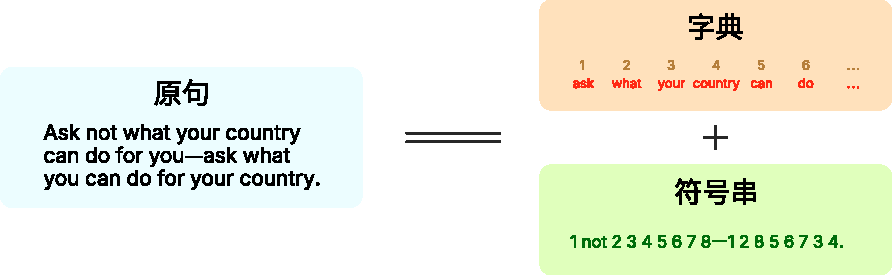
\includegraphics[width=.9\textwidth]{assets/software/Compress_a_sentence.pdf}
  \caption{压缩一个句子}
  \label{fig:Compress_a_sentence}
\end{figure}

现在,除了字典本身外,需要存储的东西就只剩极少数的几个不在字典里的单词(not、破折号和句点)以及一堆数字。在电脑里存储这样一堆符号花费的空间远远少于存储之前的那些单词,因此,即使将字典的大小也一并计算,这番操作之后的「字典」加上符号串的体积也小于原来的长句子。这个过程就是「压缩」—我们将大体积的东西无损地变成了小体积的东西,而后者可以在需要的时候变回前者。

也许你会想,这个句子长得这么对称,完全是一种特殊情况,这么做是能大幅缩减空间。那对于普通的文件,这方法也适用吗?事实上,在我们电脑上所存储的文件中——从常见的 Word 文档到各种各样的可执行文件——都包含有大量反复出现的冗余内容,完全可以用这种方式压缩。同时,当把多个文件压缩到一起时,它们中存在的重复信息亦占用了不少空间。因此,对于任意文件,我们都能通过编写「字典」,将文件转换成「符号表」。符号表和字典一同组成了「压缩文件」,转换的过程称为「压缩」,反之则称为「解压」。

\begin{figure}[htb!]
  \centering
  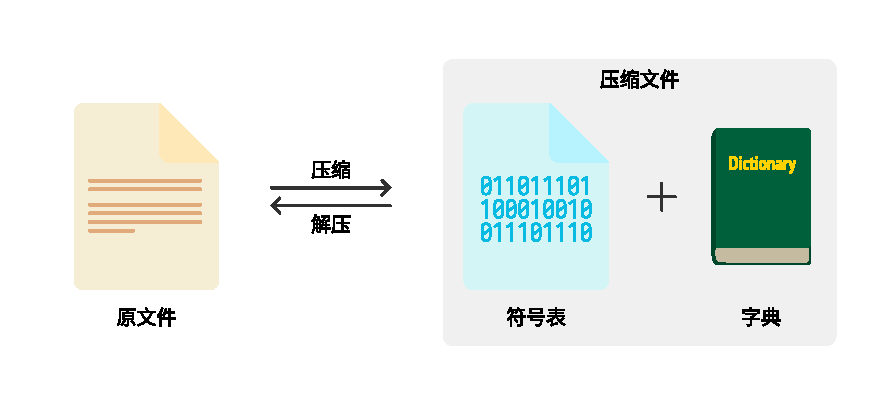
\includegraphics[width=.8\textwidth]{assets/software/Compress_and_Extract.pdf}
  \caption{压缩与解压}
  \label{fig:Compress_and_Extract}
\end{figure}

即使同为「查表替换」,具体到压缩的实现上,一千个人也可能设计出一千种方案。首先是字典生成方法的设计。我们需要明确,字典是压缩工具在「阅读」整个待压缩的文件时现场编纂的。压缩工具会以某种方式扫描所有待压缩的文件,经过一系列数学的运算后,编制出适合这些文件的高效字典。例如,上面的例子中「not」是否编入字典,就可能影响到最终的压缩效率。字典编得好不好,很大程度上决定了这个压缩策略的好坏。

另外,我们上面介绍的这种压缩是一种很笨的压缩。举个例子,相信大家都读过《汉乐府·江南》,诗是这样写的:

\begin{quoting}
  江南可采莲,\par
  莲叶何田田,\par
  鱼戏莲叶间。\par
  鱼戏莲叶东,\par
  鱼戏莲叶西,\par
  鱼戏莲叶南,\par
  鱼戏莲叶北。
\end{quoting}

看起来后面几句都有相似的结构。那么,如果把这样的一个句式作为一个字典项:

\begin{MissingVerbatim}
  鱼戏莲叶_
\end{MissingVerbatim}

其中 \MissingVerb{_} 是一个空位,可以放一些别的字进去,这样一来,压缩过程可能又可以进一步省下空间——诗的好几句都有这个句式。在文件压缩技术中,这种「能匹配长相相近片段的模板」称为「模式」(pattern)。利用好模式信息,能有效地提升压缩的效率。

这就是不同压缩文件格式(或者说种类)之间产生差异的重要原因。不同压缩文件格式有着不同的「压缩算法」,对应着不同的字典生成策略、符号替换策略,以及更多这里没有提及的技术细节。这些压缩文件格式有些技术公开,有的则并不公开;有的适用于一类特定文件,有的适用于另外许多文件。下面我们会介绍一些常用的压缩文件格式。

\section{常见的压缩文件格式}

在开始介绍这些格式之前,我们先引入一个叫做「压缩率」的概念。\regcolor{「压缩率」表示一次「压缩」操作节省了多少空间}\footnote{你可能看到有说法说「压缩率」指压缩后与压缩前的占用空间之比,但是,本文中介绍的压缩软件采用的「压缩率」均如正文中所述。}:假设一堆文件原来的总体积是 100 MB,在压缩成某种格式的压缩文件后,体积变成了 86 MB,这时的压缩率就是 $1 - 86/100 = 14\%$。压缩率不仅与压缩文件格式有关,也与源文件本身的性质有关,但我们仍然可以以「平均工作情况下的压缩率水平」的高低来笼统地比较几种不同的压缩文件格式。

\subsection{ZIP 格式——最广泛应用的格式}

ZIP 格式可以说是应用最广泛的压缩文件格式——市面上任意一款压缩工具都能制作和解压这种格式的压缩文件。即使没有安装任何压缩工具,Windows 系统也能处理这种格式的压缩包。ZIP 格式的压缩文件扩展名是 \MissingVerb{zip}。这种格式公开于 1989 年,迄今历史悠久;又由于技术细节公开,这促成了它的广泛使用。

由于诞生的时间早,现在 ZIP 格式与其他格式相比有着许多不可忽视的缺点。其最明显的缺点便是压缩率不高,这是它所使用的压缩策略决定的。然而,\regcolor{由于 ZIP 格式有广泛使用,我们仍然建议大家在与他人交换文件时,尽量使用 ZIP 格式来压缩自己的文件。}

\begin{note}
  尽管 ZIP 格式因其广泛使用而成为我们交换文件的首选,但它存在一个常见问题:它不会记录文件名的编码方式。这可能导致压缩包在解压时出现文件名乱码,尤其是在发送方和接收方使用不同操作系统的情况下。好在,目前主流的压缩工具通常能够自动检测编码来避免出现乱码。你可以阅读进阶篇的\chapref{cha:characters-and-encodings}来学习与「编码」有关的知识。
\end{note}
\subsection{RAR 格式——高压缩率的私有格式}
RAR 格式是一种压缩率比较高的压缩文件格式。它的压缩文件扩展名是 \MissingVerb{rar},这种格式诞生于 1993 年。

\regcolor{RAR 格式的技术细节是不完全公开的。}具体来说,RAR 格式的解包器是公开的,并允许以一定的方式嵌入在其他压缩工具中,而 \regcolor{RAR 格式的打包器则有专利,且完全不公开}。这意味着,市面上绝大多数压缩工具——包括我们后文介绍的几乎所有压缩工具——都不能制作 RAR 格式的压缩包,不过它们基本都能解包这种格式的压缩包。Windows 平台上的唯一能制作 RAR 压缩包的压缩工具是 WinRAR,但它要收费(可以免费试用,然而有广告)。

RAR 格式的压缩率通常比 ZIP 高上不少。除此之外,它还支持一系列其他的 ZIP 所没有的功能,例如「恢复记录」和更加安全的加密功能。鉴于制作 RAR 格式的压缩包只能使用 WinRAR,我们不太建议大家过多使用这种格式来分享文件。

\subsection{7z 格式——高压缩率的新兴开放格式}

7z 格式是一款比较年轻(相比前面两种格式而言)的压缩文件格式。它的压缩文件扩展名是 \MissingVerb{7z},这种格式诞生于 1999 年。

与 ZIP 一样,7z 格式的技术是完全公开的——这使得今天几乎所有的压缩软件都支持这种格式,无论是压缩还是解压缩。不仅如此,7z 的压缩率高于 ZIP,与 RAR 几乎平分秋色,又支持高强度加密、恢复记录等附加功能,因而 \regcolor{7z 是一种我们十分推荐个人使用的格式}。例如,如果你想将一些文件打包存档,7z 格式就是不错的选择。

然而,7z 作为后起之秀,自然没有 ZIP 或是 RAR 那样高的认可度。至少目前,在大多数人们的学习和工作中,这种格式运用得还比较少。故我们将 7z 推荐为「个人使用」——如果你想把一些文件打包发给别人(尤其是对方并不很懂电脑的情况下),ZIP 或许是更好的选择。

\section{压缩工具/压缩软件}

虽说 Windows 自身的文件管理器也能用来操作压缩软件,但它功能相对单一,操作起来不是很方便,因此我们有必要安装额外的压缩工具软件来满足使用需求。压缩工具(又称压缩软件)是一类特殊的软件。这种软件安装之后,你的电脑就可以方便地查看、解压、制作各种类型的压缩包了。

\subsection{压缩工具的使用}

\begin{wrapfigure}[8]{r}{6cm}
  \centering
  \vspace*{-1.5cm}
  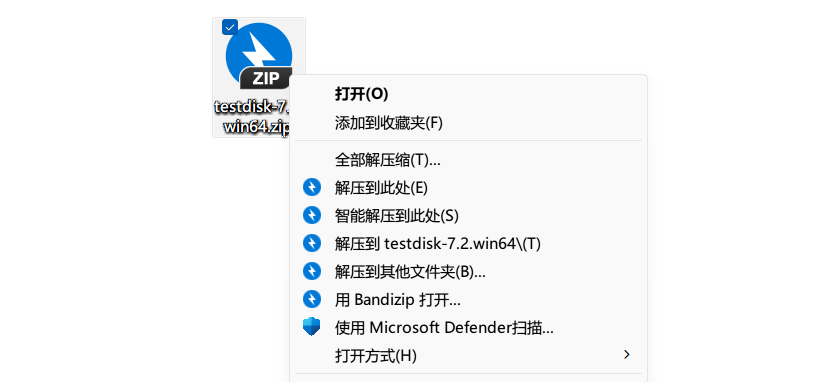
\includegraphics[width=5.5cm]{assets/software/Context_menu_of_Bandizip.png}
  \caption{Bandizip 的右键菜单}
  \label{fig:Context_menu_of_Bandizip}
\end{wrapfigure}

一般而言,压缩工具安装之后,一系列压缩文件相关的选项就会出现在文件右键菜单中。例如,当安装「Bandizip」这款压缩工具后,资源管理器的右键菜单就会多出\autoref{fig:Context_menu_of_Bandizip} 中的这些选项。

这些选项能帮助你解压和制作压缩包。例如,上图中【解压到 \MissingVerb{testdisk-7.2.win64\}】及【解压到此处】就可以将这个压缩文件解压,它们的区别早在\chapref{cha:file-and-file-management}中介绍过。而如果我们想将几个文件打包,也可以先选中它们,然后右键选择【新建压缩包】,并在弹出的窗口中选择压缩格式并设置压缩文件的名字,同时调整一些高级选项,比如给压缩文件设置密码。

\begin{figure}[htb!]
  \centering
  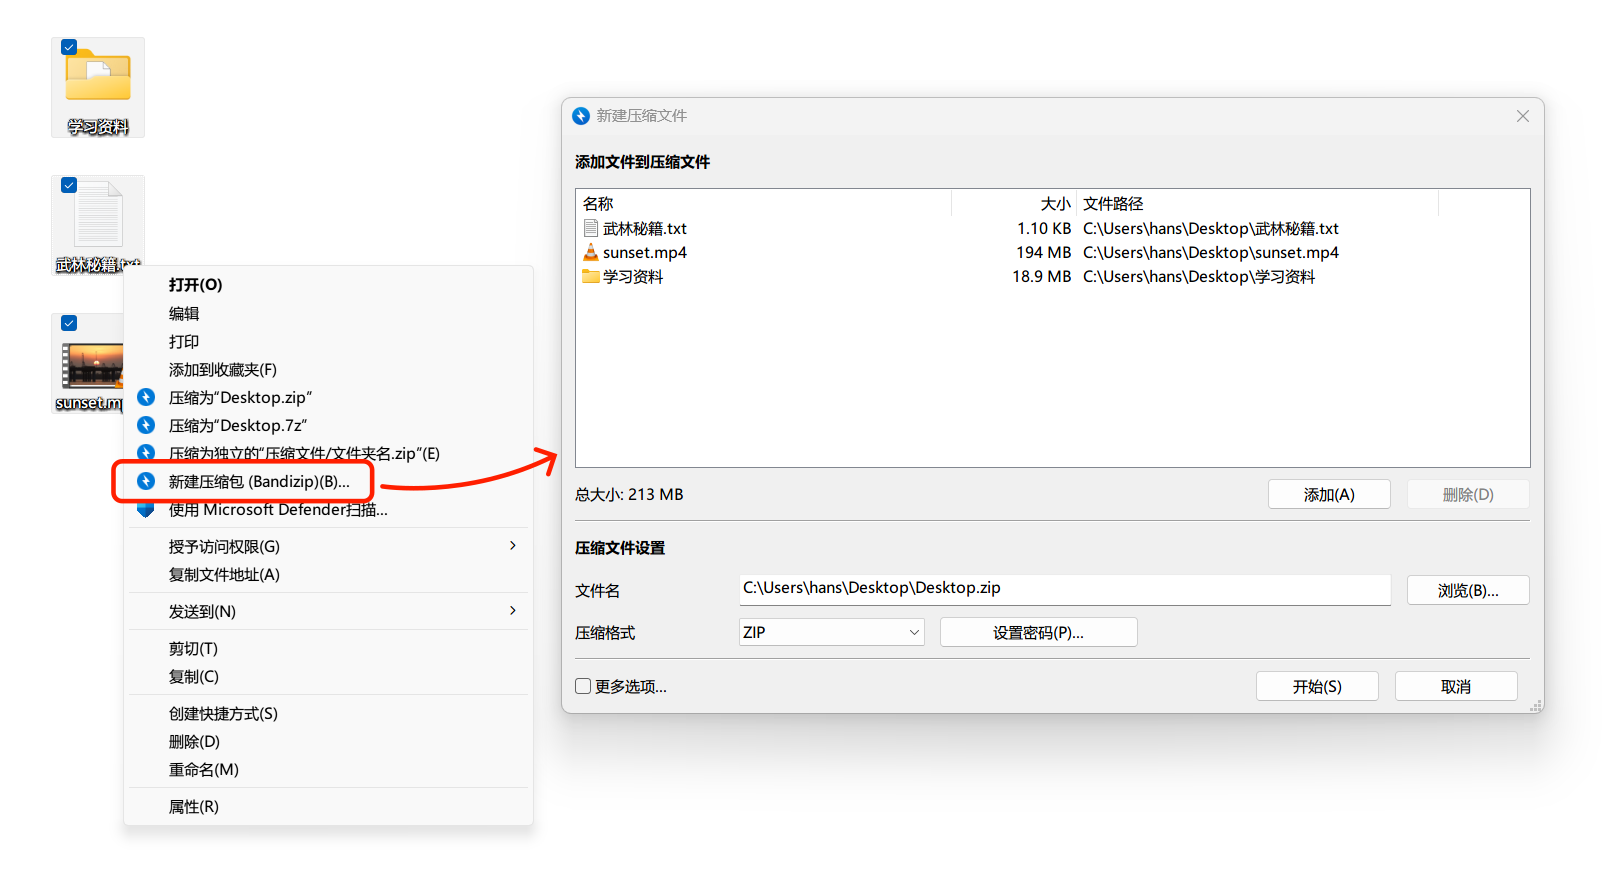
\includegraphics[width=.7\textwidth]{assets/software/Compress_with_Bandizip.png}
  \caption{用 Bandizip 新建压缩包}
  \label{fig:Compress_with_Bandizip}
\end{figure}

一般来说,双击打开一个压缩包,就可以直接查看其中的内容,而不会解包这个压缩包:

\begin{figure}[htb!]
  \centering
  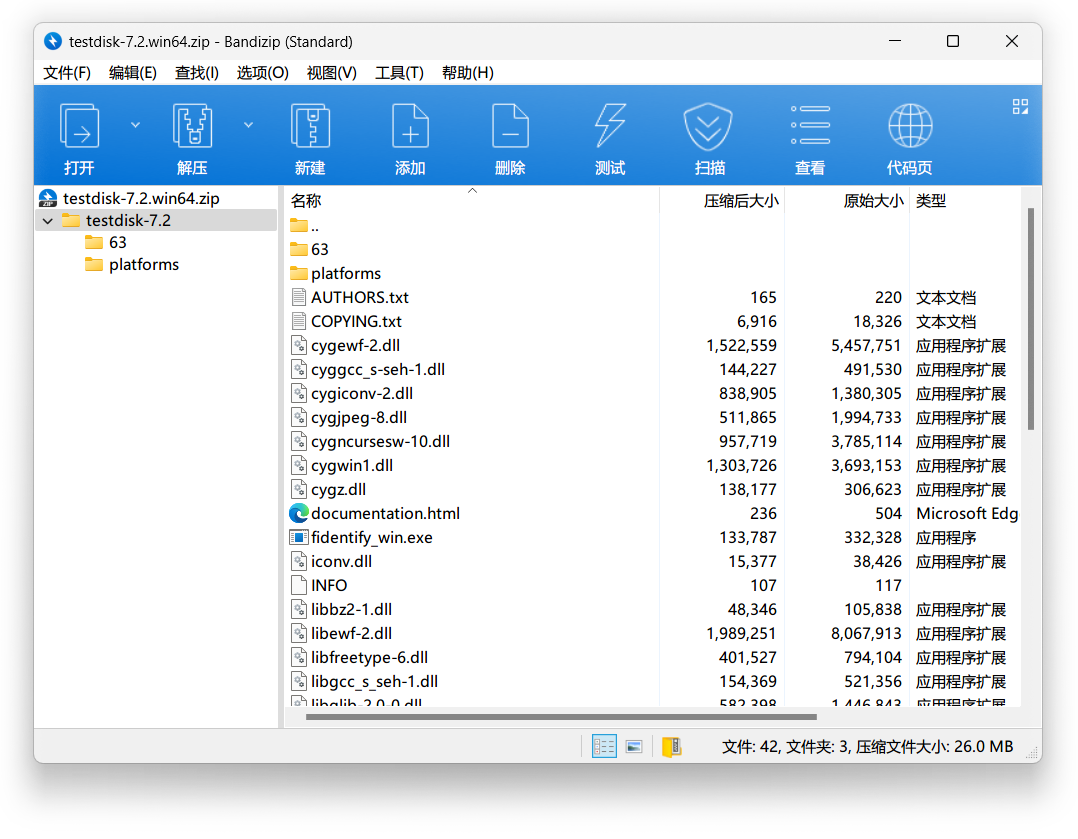
\includegraphics[width=.6\textwidth]{assets/software/Opened_archive.png}
  \caption{打开的压缩包}
  \label{fig:Opened_archive}
\end{figure}

如果你双击文件列表中的某一个文件,那么压缩工具一般只会将\regcolor{这一个文件}(而不是整个压缩包)解压到某个\regcolor{临时位置},并打开它。这一切都是临时的——在你关闭它之后,压缩工具会把这个临时文件彻底删除。因此,这种双击压缩包内某文件来打开它的方式\regcolor{只适用于临时预览压缩包中某一个文件的内容}。所以,在运行以压缩包形式提供的应用程序时,请\regcolor{一定完全解压到某个干净的地方后再运行}!

而通过拖拽,你可以将压缩包中的部分文件解压到你想要的位置。例如,如果你选中上图中的 \MissingVerb{AUTHORS.txt} 和 \MissingVerb{COPYING.txt} 两个文件及 \MissingVerb{platforms} 文件夹,然后把它们拖拽到桌面,它们就会被解压出来并放在桌面上。

\begin{note}
  压缩包也有一定的可编辑性。这意味着,借助压缩工具,你可以往已有的压缩包中继续添加新的文件,也可以删除现有压缩包中的某个文件。具体的操作依压缩工具不同而有所差异,这里不再深入介绍。
\end{note}

许多压缩格式还支持「分卷压缩」技术。假如你需要将上百个文件发送给别人,总计 1 GB,这时你首先会想到把它们压成一个略小于 1 GB 的压缩文件。然而,如果我们的聊天软件只能发送最大 200 MB 的文件,你的大压缩包就发不出去了。借助分卷压缩技术,我们可以将这总计 1 GB 的文件压缩成\regcolor{若干个不超过特定大小的「分卷压缩文件」},如下图所示。

\begin{figure}[htb!]
  \centering
  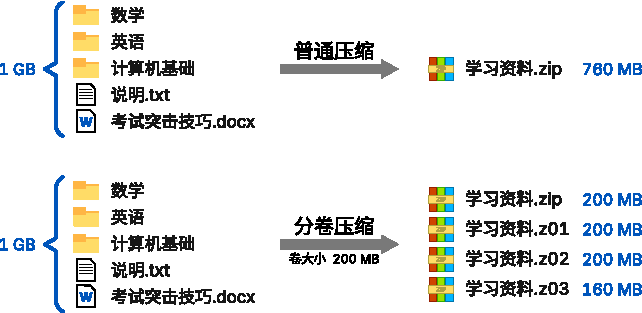
\includegraphics[width=.7\textwidth]{assets/software/Split_archive.pdf}
  \caption{分卷压缩}
  \label{fig:Split_archive}
\end{figure}

分卷压缩文件分为「主文件」与「分卷文件」,它们的扩展名与普通压缩文件有一些联系,但也有自己的规则。下面是一些常见的分卷压缩文件扩展名规则:
\begin{itemize}
  \item ZIP 格式:主文件为 \MissingVerb{zip},分卷为 \MissingVerb{z01}、\MissingVerb{z02}……
  \item RAR 格式:主文件为 \MissingVerb{part1.rar},分卷为 \MissingVerb{part2.rar}、\MissingVerb{part3.rar}……
  \item 7Z 格式:主文件为 \MissingVerb{7z.001},分卷为 \MissingVerb{7z.002}、\MissingVerb{7z.003}……
\end{itemize}

如果想要查看或解压这样的一组分卷压缩文件,只需要将它们放在同一目录下,然后操作主文件即可。压缩工具会自动找到所有的分卷并加载它们。

\begin{note}
  从上面的图中我们可以看见,所有的分卷必须有相同的主名——这正是压缩工具识别分卷的依据。如果你更改了其中一个分卷的主名,或是丢掉了其中某些分卷,解压就会失败。
\end{note}

下面,我们介绍一些常见的压缩工具。

\begin{warning}
  注意:以下列出的压缩软件均可免费使用。并且,除了 RAR 格式外,几乎所有常见的压缩文件格式都拥有公开的压缩和解压工具。因此,\regcolor{所有诱导你「开通会员」以「提高压缩速度」或「支持更多压缩格式」的压缩软件,都不值得你付费。}
\end{warning}

\subsection{资源管理器}

虽然严格来说 Windows 自己的资源管理器不算一个「压缩软件」,但我们还是在此介绍一下,用以应对别的什么压缩软件都没装的情形。

早在 Windows XP 时代,资源管理器就可以压缩与解压 ZIP 格式的压缩包。而 Windows 11 在 2023 年 11 月左右的某次更新后,它的资源管理器也可以直接打开 RAR、7z 等格式的压缩包了,倒是方便了一些;又在 2024 年下半年的某次更新后,也支持压缩为 7z 等文件了。

当资源管理器作为打开压缩文件的默认软件时,打开一个压缩包只需双击它,然后它就会在当前窗口下打开,行为看起来有点像一个普通文件夹。按理来说,它能带给用户无缝的体验,但实际上,如果压缩包里文件太多,硬盘又有点慢,那么打开压缩包(或者其内的子目录)就要卡顿好一会,性能似乎不太行。

\begin{figure}[htb!]
  \centering
  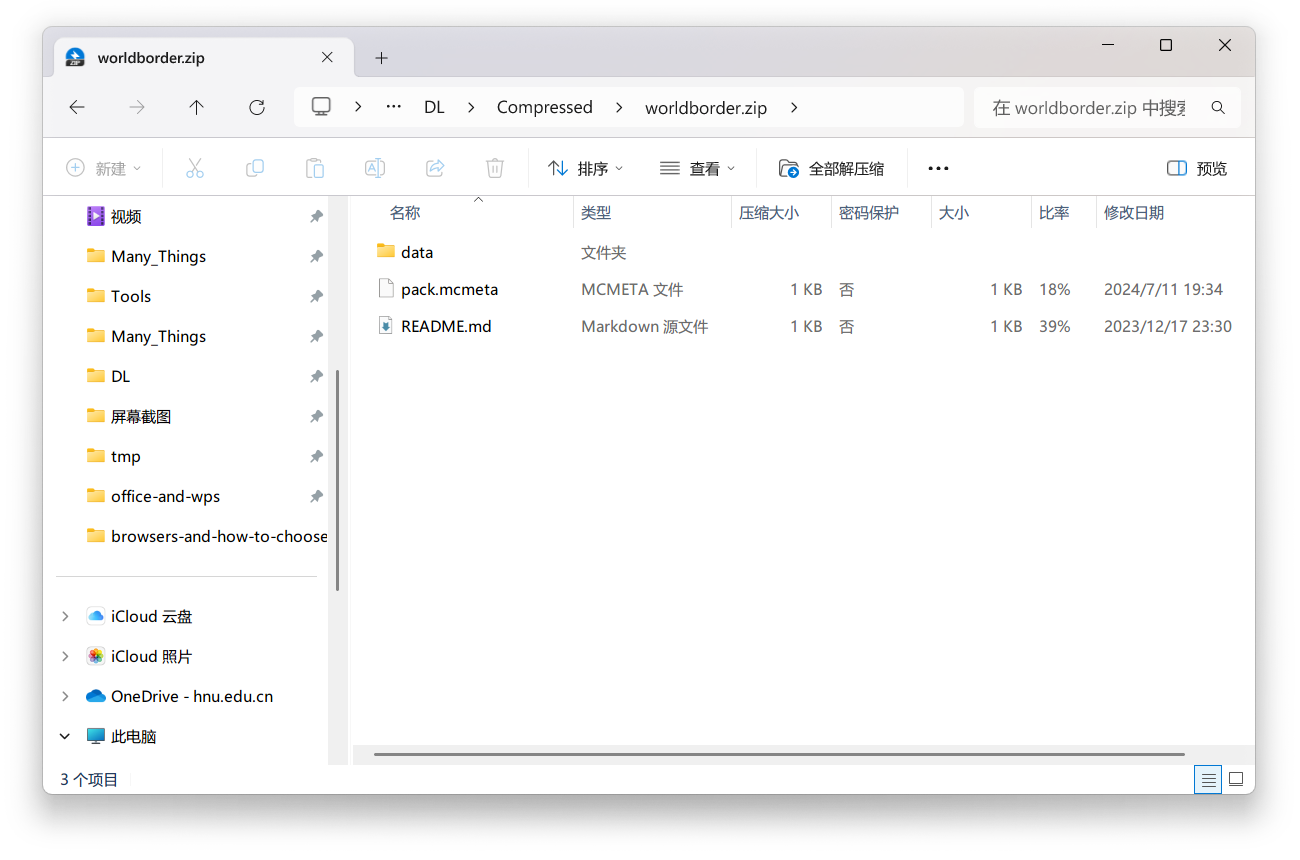
\includegraphics[width=.65\textwidth]{assets/software/explorer-open-zip.png}
  \caption{资源管理器打开压缩包}
  \label{fig:explorer-open-zip}
\end{figure}

用资源管理器解压一个压缩包只需选中压缩文件,右键 →【全部解压缩…】,然后输入解压路径即可;欲将文件压缩为 ZIP,只需选中需要压缩的文件(夹),右键 →【压缩为 ZIP 文件】,指定文件名即可。

\subsection{7-Zip/NanaZip}

7-Zip 是 7z 格式的那帮作者亲自操刀做出来的压缩工具,它是一款自由软件。除了 7z 格式之外,它还支持打开几乎所有格式(包含 RAR)的压缩包,并能制作 7z、ZIP、gzip 等各种(但不含 RAR)格式的压缩包。

7-Zip 软件比较小巧简洁,功能比较完善。其比较影响体验的缺点是外观——7-Zip 软件的默认界面风格相当的「复古」,如\autoref{fig:7-Zip} 所示。

\begin{figure}[htb!]
  \centering
  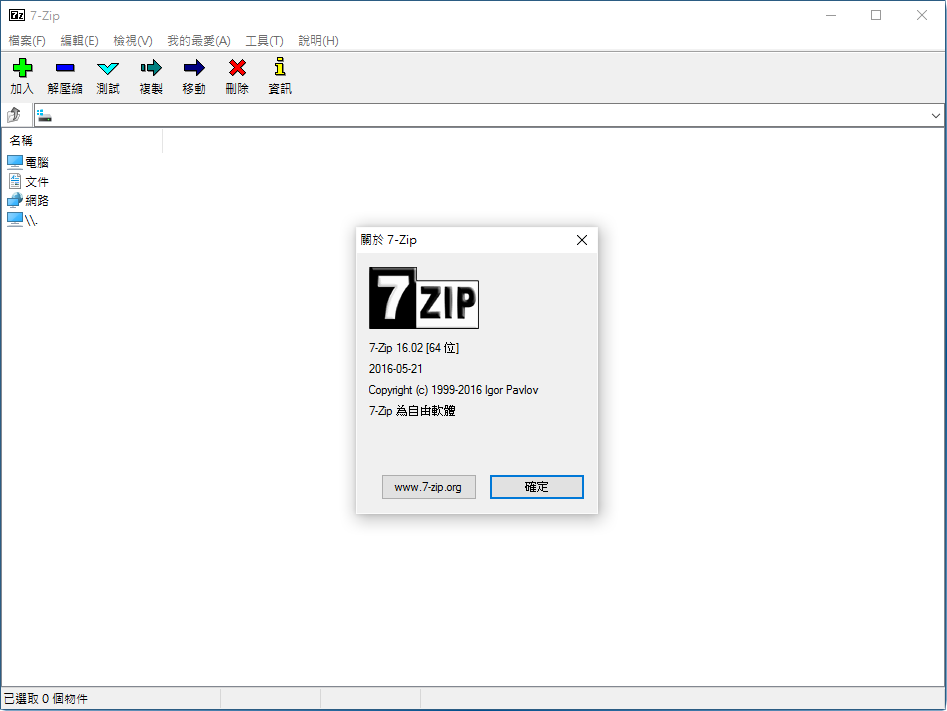
\includegraphics[width=.65\textwidth]{assets/software/7-Zip.png}
  \caption{7-Zip}
  \label{fig:7-Zip}
\end{figure}

7-Zip 的官方下载地址是 \url{https://www.7-zip.org/}。如果访问这个链接有困难,可以选择 \url{https://sparanoid.com/lab/7z/}。

由于 7-Zip 的界面复古,且不支持 Windows 11 的新式右键菜单(参见\chapref{cha:windows-11-optimization}),一些有志之士在 7-Zip 的基础上开发了 NanaZip。相比 7-Zip,NanaZip 界面简洁而现代化,并且支持 Windows 11 新式右键菜单。下面是 NanaZip 的界面。

\begin{figure}[htb!]
  \centering
  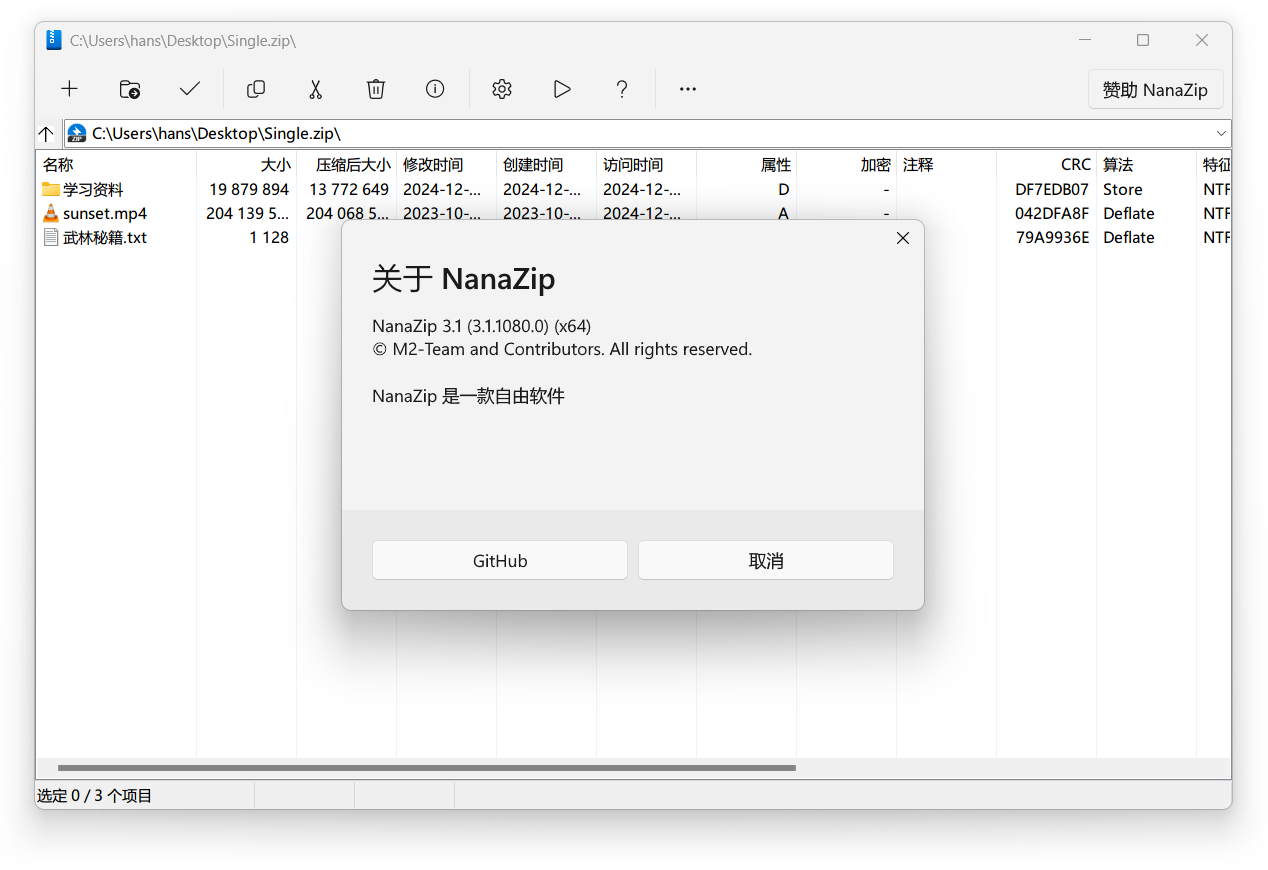
\includegraphics[width=.65\textwidth]{assets/software/NanaZip.png}
  \caption{NanaZip}
  \label{fig:NanaZip}
\end{figure}

NanaZip 可以在 Microsoft Store 搜索「NanaZip」直接安装。或者,你也可以在 \url{https://github.com/M2Team/NanaZip/releases} 手动下载安装它。

\subsection{Bandizip}

Bandizip 是由 Bandisoft 开发的一款压缩软件,有免费的标准版与付费的专业版、企业版。它也支持读取几乎所有格式的压缩包,也能制作包括但不限于 ZIP、7z 等格式的压缩包。当然,和 7-Zip 一样,Bandizip 无法制作 RAR 压缩包。

Bandizip的主界面大致如下图所示。可以看见,它的界面较为简洁、现代,但美中不足的便是右下角的广告。这广告需要我们购买专业版或企业版才能去除。

\begin{figure}[htb!]
  \centering
  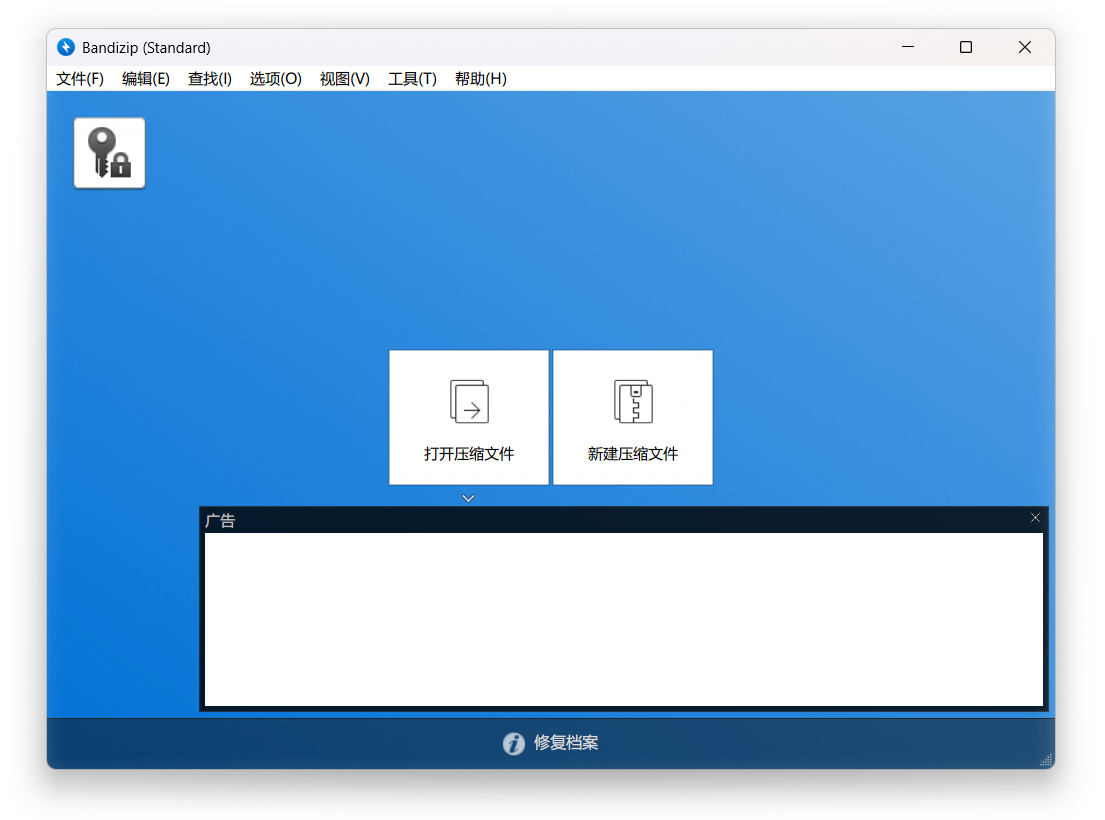
\includegraphics[width=.55\textwidth]{assets/software/Bandizip_main_window.png}
  \caption{Bandizip}
  \label{fig:Bandizip_main_window}
\end{figure}

此外,在 2025 年 2 月的某次更新后,Bandizip 的免费版会每隔两三天,在当天第一次运行软件(无论是打开、压缩还是解压压缩包)的时候,从屏幕的右下角弹出一些广告,如下图所示,它同样也需要购买专业版或企业版去除。虽然广告的内容不像下文的 WinRAR 那样离谱,但仍对我们的使用体验造成了不小的打击。

\begin{figure}[htb!]
  \centering
  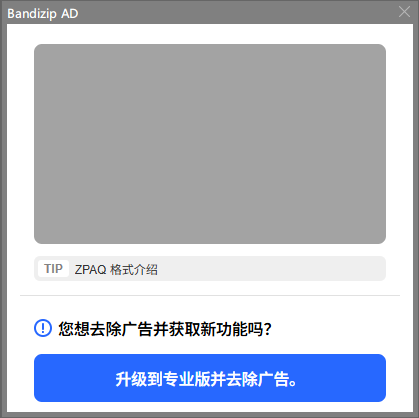
\includegraphics[width=.45\textwidth]{assets/software/Bandizip_popup.png}
  \caption{Bandizip}
  \label{fig:Bandizip_popup}
\end{figure}

当你使用 Bandizip 打开一个压缩文件时,软件界面大致如下图,你可以在此对压缩文件进行各种操作。

\begin{figure}[htb!]
  \centering
  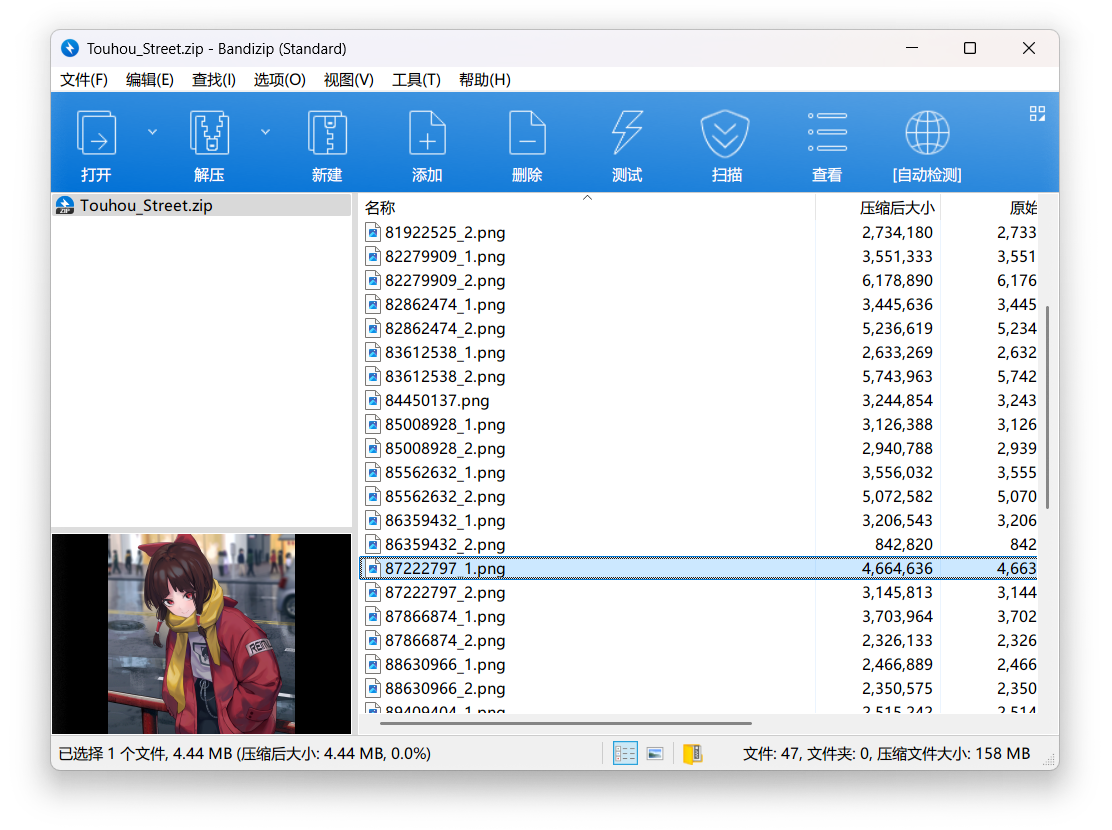
\includegraphics[width=.65\textwidth]{assets/software/Bandizip_opening_archive.png}
  \caption{用Bandizip打开文件}
  \label{fig:Bandizip_opening_archive}
\end{figure}

Bandizip 值得一提的两个功能,一是「压缩文件预览」,二是「智能解压」。

「压缩文件预览」是说,当你右击一个压缩文件时,若这个文件没有加密文件名\footnote{对于一般的加密压缩文件,即使我们手中没有密码,仍然可以查看其中的文件列表;但如果在加密时选择了加密文件名,那么没有密码的情况下,连文件列表也无法查看。},你的右键菜单便会显示出这个压缩包内部的部分文件;若是连文件名都加密了,那当然什么都看不见啦。这个功能默认未启用,需要在 Bandizip 的【设置】→【上下文菜单】→【选择解压菜单】中开启。但这个功能只支持旧式菜单,不支持 Windows 11 的新式菜单。

\begin{figure}[htb!]
  \centering
  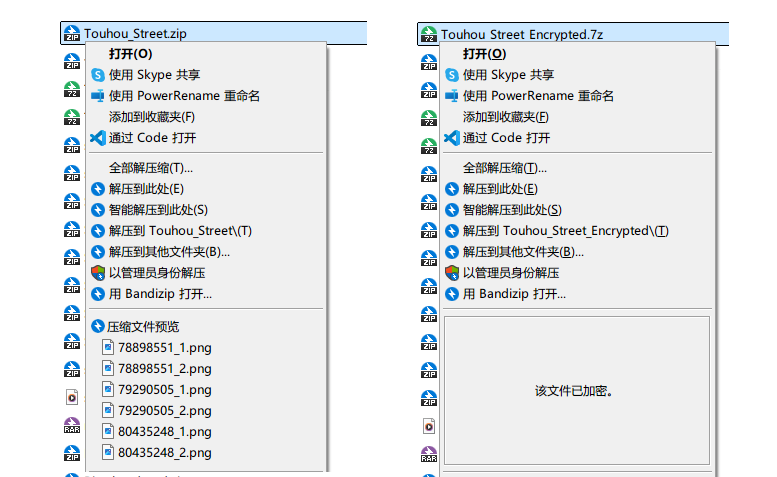
\includegraphics[width=.7\textwidth]{assets/software/Compressed_Preview.png}
  \caption{右键菜单中的「压缩文件预览」}
  \label{fig:Compressed_Preview}
\end{figure}

「智能解压」则是一种「傻瓜式解压操作」。还记得\chapref{cha:file-and-file-management}中我们介绍的「解压到当前文件夹」和「解压到 \MissingVerb{<文件名>\}」的区别吗?「智能解压」能够自动在这两种模式中选择更合适的那个——当你的压缩文件根目录仅有一个项目(无论文件或文件夹)时,Bandizip 会选择前者;若有多个项目, Bandizip 则会选择后者。

举个例子:上图中的压缩包内部就有许多图片,假设这个压缩包的路径是 \MissingVerb{D:\Touhou_Street.zip},点击【智能解压到此处】之类的选项,那么图片就会被提取到 \MissingVerb{D:\Touhou_Street\} 下;若这压缩包里面就一张图,则会被提取到 \MissingVerb{D:\} 下。

智能解压既支持旧式右键菜单也支持 Windows 11 的新式右键菜单,若使用 Bandizip,我们建议你使用智能解压来解压文件,这样就不用担心会弄乱自己的工作目录了。

\begin{figure}[htb!]
  \centering
  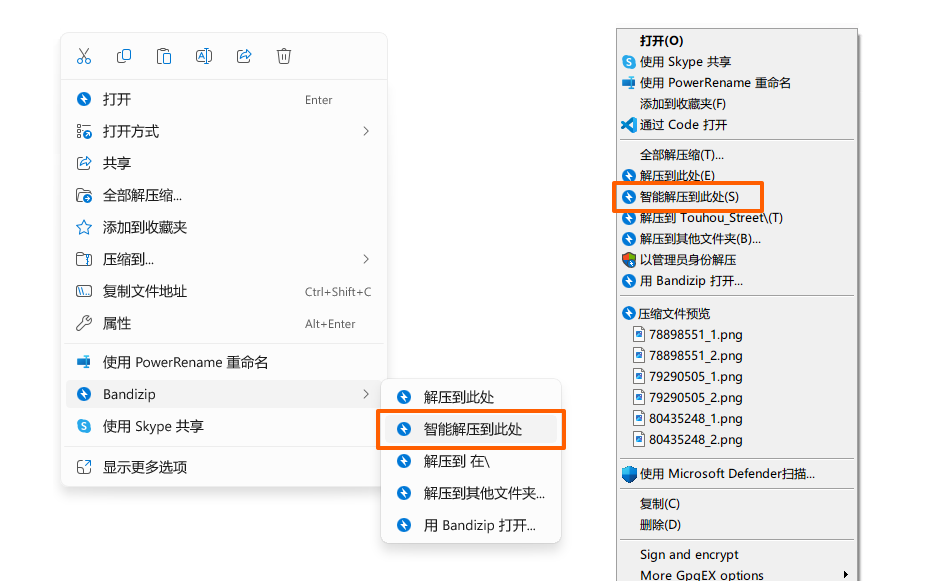
\includegraphics[width=.8\textwidth]{assets/software/Smart_Extract.png}
  \caption{「智能解压」右键菜单}
  \label{fig:Smart_Extract}
\end{figure}

Bandizip 免费版可以在 \url{https://www.bandisoft.com/bandizip/} 下载到,如果你能忍受不时出现的小广告,那么它的使用体验还算不错。

\subsection{WinRAR}

WinRAR 是 RAR 格式的作者设计的软件。顾名思义,WinRAR 最大的特点就是「RAR」——它(可能)是 Windows 平台上唯一一款能够支持制作 RAR 格式压缩包的压缩软件。除了 RAR 格式外,它也支持其他各种压缩格式的压缩和解压。WinRAR 的软件界面如下图所示。

\begin{figure}[htb!]
  \centering
  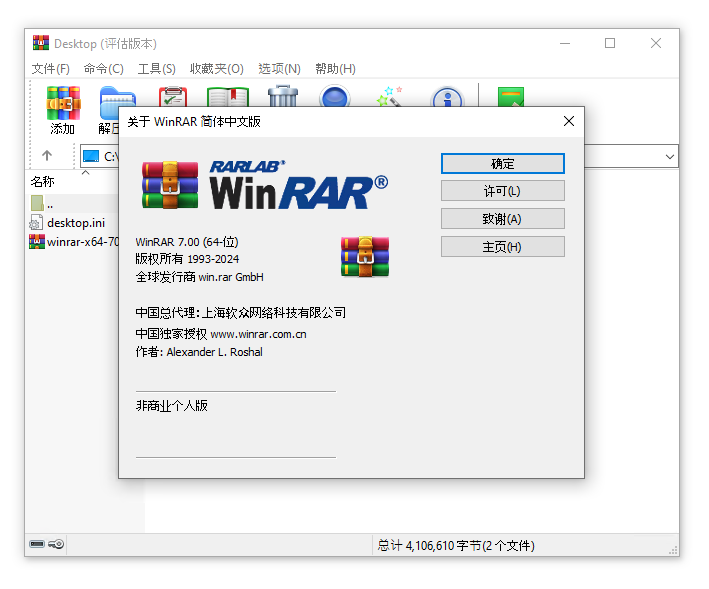
\includegraphics[width=.7\textwidth]{assets/software/WinRAR_main_window.png}
  \caption{WinRAR}
  \label{fig:WinRAR_main_window}
\end{figure}

WinRAR 是收费的商业软件——换言之,这款软件需要购买才能使用。不过,WinRAR 在中国也提供了一个「个人免费版本」,这个版本包含恶性弹窗广告——与 Bandizip 那种不同,WinRAR 的广告在打开压缩文件的时候也会弹出。如果你能接受那样的弹窗广告,那么 WinRAR 也许是一个不错的选择。

\begin{figure}[htb!]
  \centering
  
\includegraphics[width=.5\textwidth]{assets/software/WinRAR_ad.png}
  \caption{WinRAR 的弹窗广告}
  \label{fig:WinRAR_ad}
\end{figure}

WinRAR 的国际官网是 \url{https://www.rarlab.com/},但如果要下载「个人免费版」,请访问 WinRAR 国内代理官网 \url{http://www.winrar.com.cn/index.htm}。

\subsection{国产压缩软件}

最后我们来介绍一下压缩软件中的「深水区」——国产压缩软件们。和\chapref{cha:browsers-and-how-to-choose} 一样,国产压缩软件也良莠不齐,其中不乏佳作也不少恶意软件。由于除了 RAR 之外的几乎所有压缩格式都是公开的,因此几乎所有的国产压缩软件都和前文介绍的 7-Zip 或 Bandizip 一样,支持绝大多数格式压缩文件的解压,但不支持 RAR 格式压缩文件的制作。例如,下面是「360 压缩」的客服人员对「『360 压缩』能否压缩 RAR 格式」这一问题的答复:

\begin{figure}[htb!]
  \centering
  
\includegraphics[width=.9\textwidth]{assets/software/360Zip_not_supporting_rar_compress.png}
  \caption{「360 压缩」能否压缩 RAR 格式?}
  \label{fig:360Zip_not_supporting_rar_compress}
\end{figure}

与「360 压缩」这种「还算好用」的国产压缩软件相比,有些软件等则表现出了许多恶意软件的特征——静默捆绑安装、大量的广告推送,以及难以卸载和清除。同时,一些国产压缩软件还推出了各种所谓的「会员」功能,用于所谓「去除广告」「提升解压速度」「支持更多压缩格式」等,为这些原本就是免费的内容付费,实无任何必要。

总而言之,和前文介绍浏览器时我们的态度一样,对于国产压缩软件,我们建议各取所需,审慎行事。

\practice

\begin{enumerate}
  \item 用自己的话简要复述「压缩」这个过程。
  \item 自己制作几个压缩文件,然后分别用「解压到当前文件夹」「解压到 \MissingVerb{<文件名>\}」来解压它们,体会这两种解压方式的区别。思考 Bandizip 的「智能解压」到底有多智能。
  \item 你正在使用什么压缩软件?它的使用体验(界面美观度、操作难易度、是否有广告……)如何?
\end{enumerate}